\section{Results}
    \subsection{Data Exploration}
        During the data exploration, the dataset has been fully created and all of the features have been visualized. 
        %Most of the data seems to be strongly right skewed, for example, take a look at Figures \ref{fig:avg-follower-contributor-plot} - \ref{fig:nr-commit-contributor-plot}.
        %However, there are also plots that did not have this right skew property.
        %These will be explained in more detail, as they require some more understandig of the data.
        Most of the features are extremely right skewed; these have not been displayed graphically but can be found in Figure \ref{fig:right-skewed-features}. This table displays the minimum, maximum, mean and median value for each of the features.
        It can be easily seen that the average is always higher than the median, which is an indication that the data is right skewed.
        However, other features did give more interesting insights; this involves mostly the categorical variables. 
        This report does include a visualisation of those features, as well as an explanation as they might require some deeper understanding of the data.
        
        \begin{figure}[h!]
	        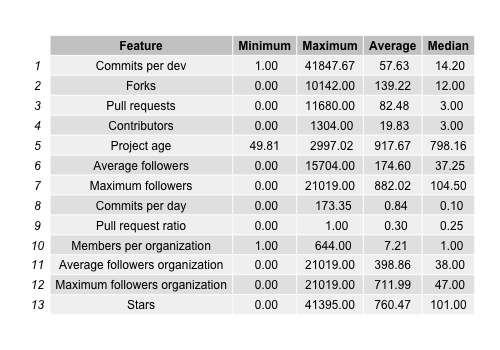
\includegraphics[width=250pt]{figures/data_summary_table}
	        \caption{The minimum value, maximum value, mean and median of all the right skewed variables}
	        \label{fig:right-skewed-features}
	    \end{figure}
        
    	\begin{LaTeXdescription}
    	\item[Countries]
    	Figure \ref{fig:country-plot} shows the countries in which the project was created.
    	As can be easily retrieved from the figure, most of the projects tend to be created in the US.
    	However, we also find a large spike for the `unknown' value, which indicate that a lot of the developers on GitHub have not specified their country of origin.
    	\item[Programming languages]
    	Figure \ref{fig:language-frequency-plot} shows the programming languages used in each of the projects in the dataset.
    	Just as with the countries, we see a big spike for the `unknown' value.
    	The reason behind this is that there are a lot of projects on GitHub that are created, but do not have any commits.
    	It is then not possible for GitHub to define a language for the project, thus we get an entry with `unknown'.
    	\item[Forks]
    	A project can be either created by a GitHub user, or be forked from an existing project.
    	Because forks tend to behave differently, for example they keep the amount of forks the original project has on GitHub, but do not get the same amount of stars, a histogram was made to see how many of the projects in the dataset are a fork.
    	This histogram can be found in Figure \ref{fig:is-fork-plot} and shows that most of the projects are not a fork.
    	\item[Project age]
    	The age of the projects can be found in Figure \ref{fig:age-plot}.
    	The age is defined as the amount of days from initial created, until January 6, 2016.
    	As can be seen from the figure, there are more projects recently created.
    	This is also in line with what you would expect, as GitHub tends to grow each year \cite{github-2013}.
    	\item[Ratio of accepted pull requests]
    	Figure \ref{fig:ratio-pull-requests-plot} shows the percentage of pull requests that was accepted per project.
    	There are two things in this plot that might attract your attention: most of the projects have a percentage of 0 accepted pull request, and there is an increase at 1 (or 100\%). 
    	Both can be easily explained: a lot of projects have a small amount of pull requests of which none are accepted, which explaints the spike around 0.
    	On the other hand, a lot of project also have one or two pull requests and have accepted these, which means that they accepted all of them.
    	Since the majority of the projects fall in these two categories, there is also an increase around 100\%.
    	\item[Number of commits per contributor]
    	Although Figure \ref{fig:nr-commit-contributor-plot} looks like a normal right skewed histogram, there is some information missing in this figure.
    	When creating the data for this plot, it was necessary to divide the amount of commits by the amount of contributors.
    	However, there can be so called `read-only mirrors' on GitHub that have commits without any contributors (for example https://github.com/cran/jomo).
    	When dividing the amount of commits by the amount of developers, this result in a division by 0 which was represented as infinity.
    	These values were not added in the plot. 
    	\item[Domains]
    	Figure \ref{fig:project-domain-plot} shows the domains and the amount of projects that were classified into that domain.
    	This classification was done manually and is based on the top level domains of the 2012 ACM classification \cite{acm-2012}.
    	In addition, two other domains were added - \textit{empty} and \textit{not found} - which respectively indicate that a certain project did not contain any files and that a project could not be found anymore on GitHub.
    	\end{LaTeXdescription}
        
	    %\begin{figure}[t!]
	    %    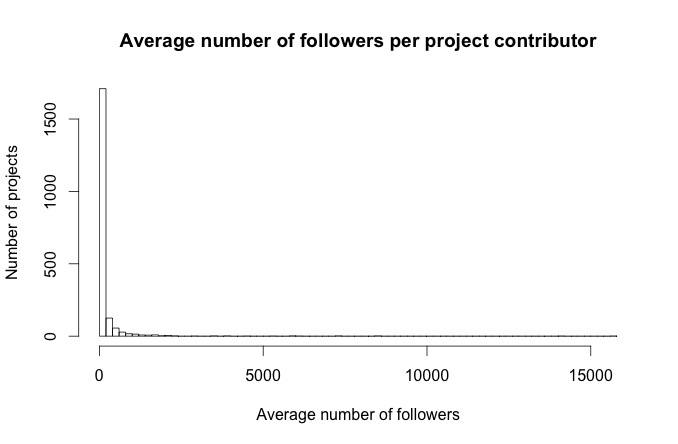
\includegraphics[width=250pt]{figures/average-number-of-followers-per-project-contributor}
	    %    \caption{The average number of followers per project contributor}
	    %    \label{fig:avg-follower-contributor-plot}
	    %\end{figure}

%	    \begin{figure}[t!]
	  %      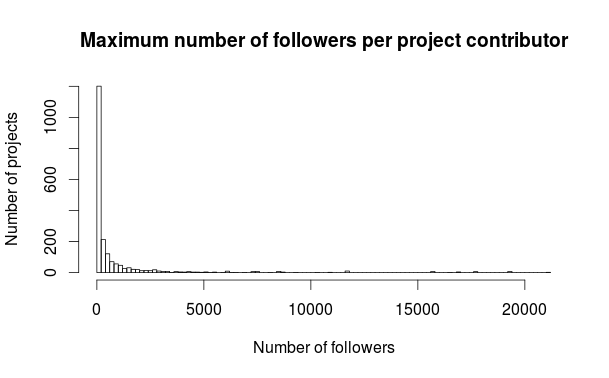
\includegraphics[width=250pt]{figures/maximum-number-of-followers-per-project-contributor}
	  %      \caption{The maximum number of followers per project contributor}
	  %      \label{fig:max-follower-contributor-plot}
	  %  \end{figure}

	   % \begin{figure}[t!]
	   %     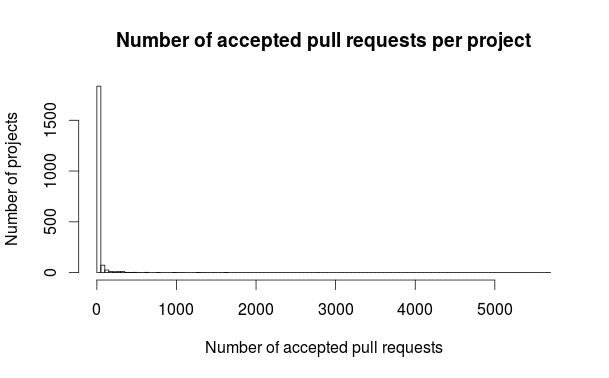
\includegraphics[width=250pt]{figures/nr-of-accepted-pull-requests-per-project}
	   %     \caption{The number of accepted pull requests per project}
	   %     \label{fig:accepted-pull-plot}
	   % \end{figure}

	   % \begin{figure}[t!]
	   %     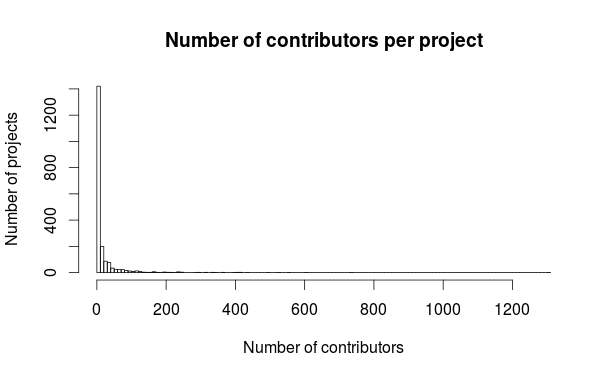
\includegraphics[width=250pt]{figures/nr-of-contributors-per-project}
	   %     \caption{The number of contributors per project}
	   %     \label{fig:nr-contributors-plot}
	   % \end{figure}

	   % \begin{figure}[t!]
	   %     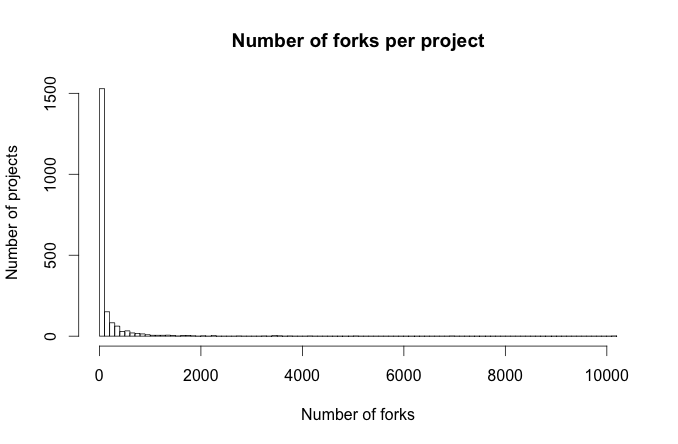
\includegraphics[width=250pt]{figures/number-of-forks-per-project}
	   %     \caption{The number of forks per project}
	   %     \label{fig:nr-forks-plot}
	   % \end{figure}

	   % \begin{figure}[t!]
	   %     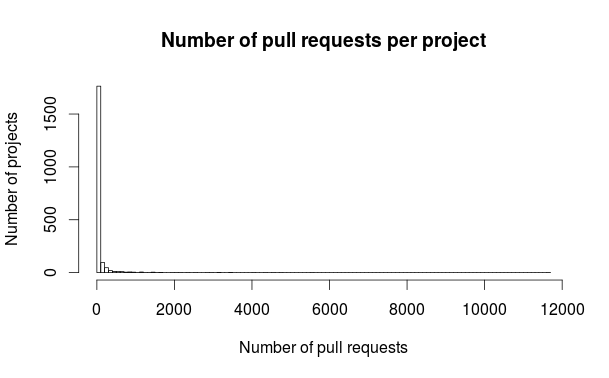
\includegraphics[width=250pt]{figures/number-of-pull-requests-per-project}
	   %     \caption{The number of pull requests per project}
	   %     \label{fig:nr-pull-requests-plot}
	   % \end{figure}

	   % \begin{figure}[t!]
	   %     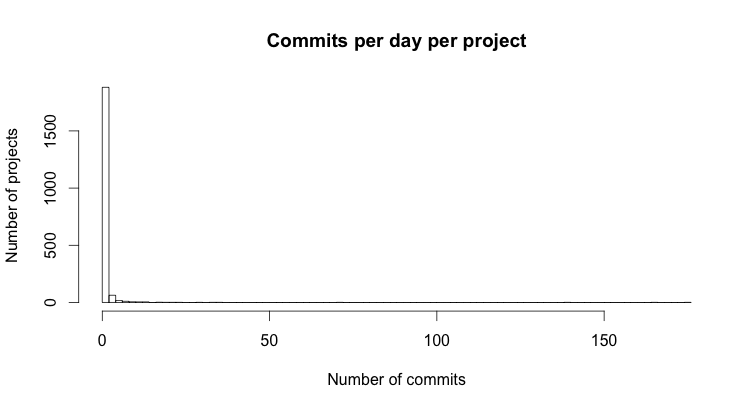
\includegraphics[width=250pt]{figures/commits-per-day-per-project}
	   %     \caption{The number of commits per day per project}
	   %     \label{fig:nr-commits-day-plot}
	   % \end{figure}

	    \begin{figure}[h!]
	        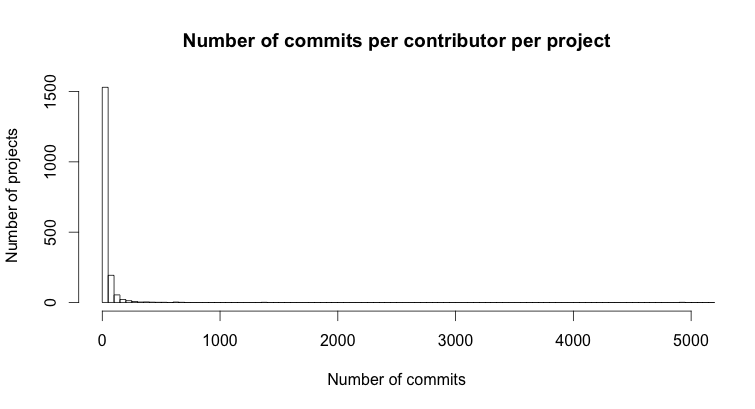
\includegraphics[width=250pt]{figures/nr-commits-per-contributor}
	        \caption{The number of commits per contributor per project}
	        \label{fig:nr-commit-contributor-plot}
	    \end{figure}

	    \begin{figure}[h!]
	        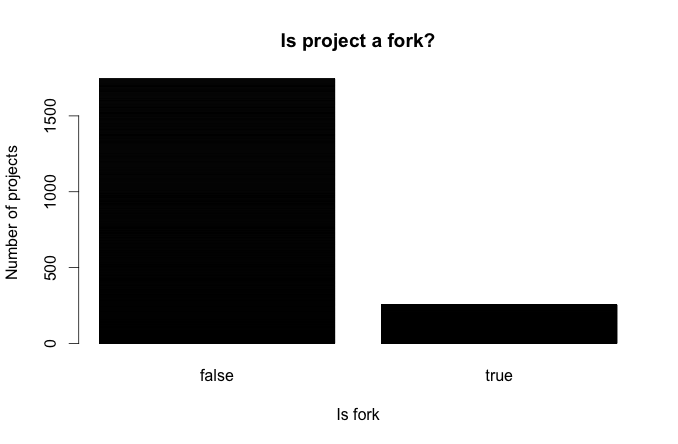
\includegraphics[width=250pt]{figures/isfork-per-project}
	        \caption{A histogram showing whether a project is a fork or not}
	        \label{fig:is-fork-plot}
	    \end{figure}

	    \begin{figure}[h!]
	        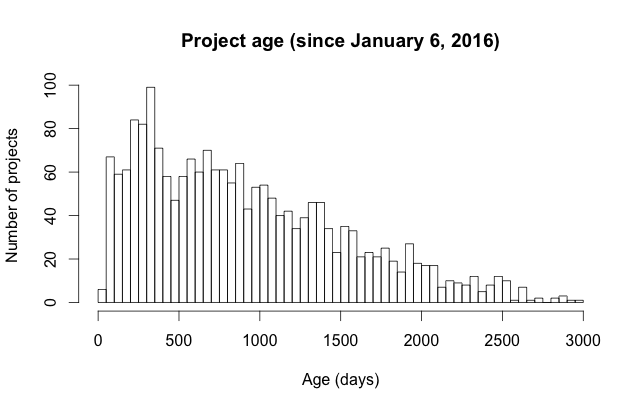
\includegraphics[width=250pt]{figures/project-age}
	        \caption{The age of the project in days from January 6, 2016}
	        \label{fig:age-plot}
	    \end{figure}

	    \begin{figure}[h]
	        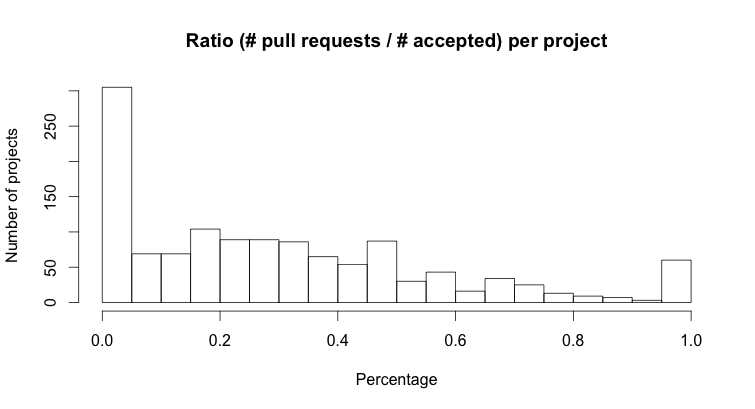
\includegraphics[width=250pt]{figures/ratio-pull-request-per-project}
	        \caption{The ratio of accepted pull requests per project}
	        \label{fig:ratio-pull-requests-plot}
	    \end{figure}

	    \begin{figure*}[t!]
	        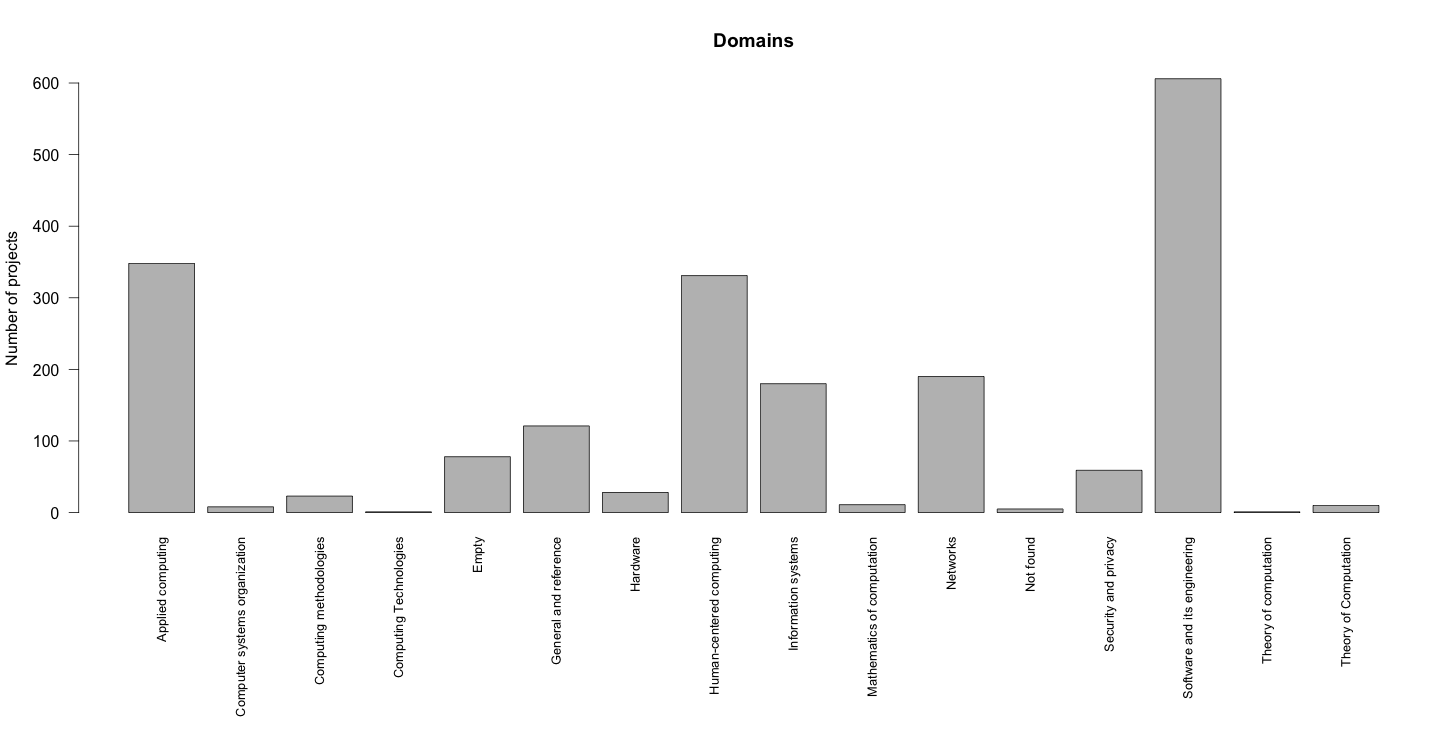
\includegraphics[width=500pt]{figures/project-domains}
	        \caption{An overview of the amount of projects per domain}
	        \label{fig:project-domain-plot}
	    \end{figure*}

	    \begin{figure*}[t!]
	        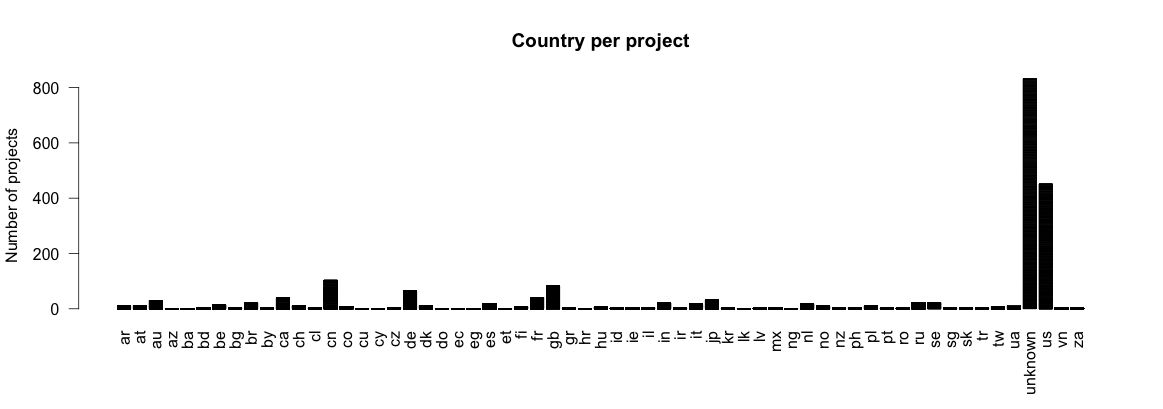
\includegraphics[width=500pt]{figures/country-per-project}
	        \caption{An overview of the countries where the project was created}
	        \label{fig:country-plot}
	    \end{figure*}

	    \begin{figure*}[t!]
	        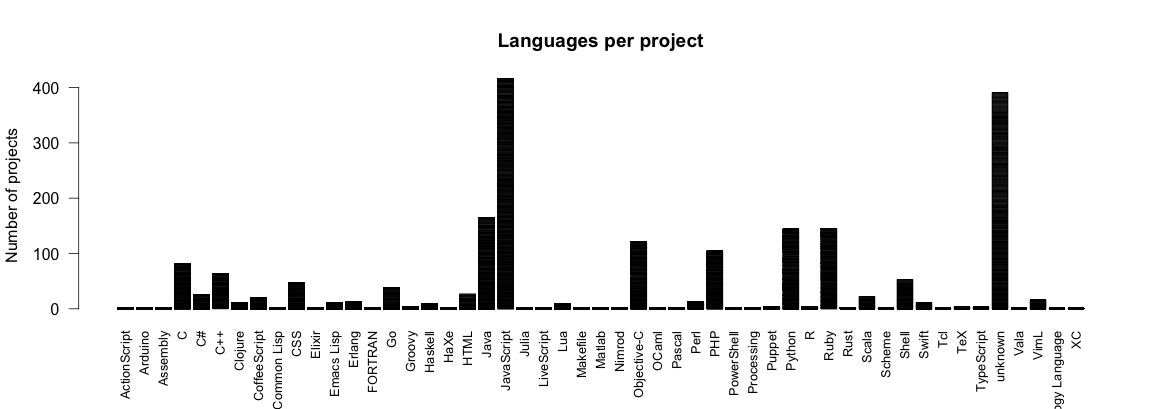
\includegraphics[width=500pt]{figures/languages-per-project}
	        \caption{An overview of the languages user per project}
	        \label{fig:language-frequency-plot}
	    \end{figure*}
    
    \subsection{Relations}
    Better understanding of the different features was achieved by plotting the correlations.
    The result of using spearman's rank correlation coefficient \todo{reference} on the sampled data can be found in Figure \ref{fig:correlation-plot}.
    When examining the created plot, there were some interesting relations found.
    The first one was the negative correlation between the age of a project and its id.
    This was not very surprising, as the ids of the older projects are lower as these were added to the GHTorrent dataset first.
    Another notable thing is that the average followers per organization and maximum followers per organization - and the same applies to average followers and maximum followers of contributors - were strongly correlated. 
    Lastly the number of pull request seems to be strongly correlated to the amount of contributors.
    Again this is not surprising, as a contributor is someone that contributed to the project. 
    Since this can only be done by using a pull request, if you are not one of the core developers, the amount of pull requests is influenced by the amount of people that have contributed to a project.
    \begin{figure}[h!]
	    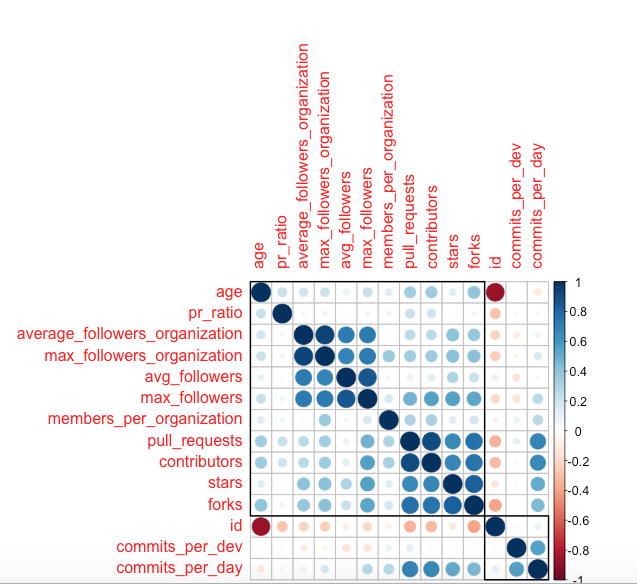
\includegraphics[width=250pt]{figures/correlation}
	    \caption{Correlation between the different features}
        \label{fig:correlation-plot}
	\end{figure}

    \subsection{Testing the model}
        After sufficient insight in the features and the relations between the features was gained, a model was created. 
        This model consists of the dependent variable, stars, and has almost all the features listed earlier as features. 
        Based on the exploration, it was decided to drop three variables: the maximum number of followers per organization, the average number of followers per contributor and the pull request acceptance ratio.
        As stated earlier, the features concerning followers were closely related, so it was decided to keep half of them. 
        The pull request acceptance ratio was dropped because of the many repositories that did not had any pull requests at all. 
        This made a lot of entries in our feature table not usable, as it lacked information. 
        To overcome this problem, the pull request acceptance ratio was removed from the model.
        
        Several algorithms have been used to train the model. 
        The results can be found in table \ref{table:r-squared-table}.
        All the algorithms were run on several versions of the dataset. The first version contained just the values that were retrieved from the GHTorrent dataset, and is indicated by `normal'. 
        In the `scaled' version, all numerical features are scaled such that the mean is equal to zero and the standard deviation is equal to one. 
        The last version is the `log-scaled' version. \todo{Each value in each numerical feature has been replaced by the value that was retrieved from taking the natural logarithm of each value; however, due to the fact that $log(0)$ is undefined and almost all numerical features contain zeroes, each value was first increased by 1. VERBETER DEZE ZIN :)}.
        Each `N/A' entry in the table means that the algorithm could not be run on that dataset, or that it did not yield useful result.
        Two algorithms that have been tried are not shown in the table; both Multiple Linear Regression and General Linearized Model did not provide useful results on any of the versions of the datasets.
        
        \begin{center}
        \begin{tabular}[width=250pt]{|l|c|c|c|}

            \hline
            Algorithm                   & normal    & scaled   & log-scaled \\ \hline
            %Multiple Linear Regression  &    N/A    & N/A      & N/A                \\ 
            PCR                         &   0.55    & 0.63     & 0.87          \\
            PLSR                        &   0.52    & 0.47     & 0.86          \\
            Stepwise Linear Regression  &   0.53    & 0.58     & 0.05         \\
            %GLM                         &   N/A     & N/A      & N/A               \\
            Neural Networks             &   N/A     &   0.24   & N/A               \\
            Random Forest\footnotemark  &   0.57    & 0.58     & \textbf{0.88} \\
            \hline
        \end{tabular}
        \captionof{table}{Mean r-squared values for several algorithms used on different versions of the dataset}
        \label{table:r-squared-table}
        \end{center}
        \footnotetext{In order to make this algorithm work, the country of origin feature was removed, as the implementation that was used was not able to handle a categorical variable with such a large number of possible values.}
        
        
        It is interesting to see that 3 out of 4 algorithms performed best on the `log-scaled' version of the dataset. A possible explanation is that most of the chosen algorithms may perform better when there are no negative values involved. The scaled version of the dataset does contain negative values, where the logarithmically scaled version does not, because each value was first increased by one.
        
        The best $R^2$ was achieved by the Random Forest algorithm on the logarithmically scaled dataset, with $R^2 = 0.88$. This means that 88\% of all the variance between the predictions made by the model and the actual dataset can be explained, and is due to variance in the dataset itself; the other 12\% cannot be explained and is caused by the fact that the model is not perfect and cannot match the reality exactly.
        \todo{EXPLAIN WHY RANDOMFOREST WORKS WELL: because of majority votes. ADD REFERENCE TO RANDOMFOREST THING}
                
        It was also tried to extract all the items with a certain domain, e.g. `Networks' and run the various algorithm on a dataset containing just objects with just that domain. However, this did not yield any valuable results. 
        The best $R^2$ value for those tests was 0.39, which means that still 61\% of the variance between the model and the actual data could not be explained.
        
    \subsection{Important features}
        As is clear from the results shown earlier, it is possible to predict the number of stars of a project relatively accurately. 
        The follow-up question is: which features from the dataset are most important in this prediction? 
        Table \ref{table:inc-mse-feature-removal} shows the increase in the Mean Squared Error when a certain feature is removed from the model.
        \begin{center}
        \begin{tabular}[width=250pt]{|p{5cm}|c|}
            \hline
            Feature                                                       & MSE increase (\%) \\
            \hline
                Number of forks                                            & 53.9     \\
                Average number of followers per organization member        & 26.6    \\
                Number of pull requests                                    & 25.2     \\
                Average number of commits per day                          & 19.3     \\
                Maximum number of followers per contributor                & 18.9                   \\                    
                Number of contributors                                     & 16.5      \\
                Project age                                                & 16.3  \\
                Project is a fork                                          & 13.0      \\
                Language                                                   & 12.1      \\
                Average number of commits per developer                    & 11.4         \\
                Project has a description                                  & 8.0 \\
                Domain                                                     & 5.3 \\
                Number of members of organization                          & 4.3 \\
            \hline
        \end{tabular}
        \captionof{table}{Increase in MSE when a feature is removed}
        \label{table:inc-mse-feature-removal}
     \end{center}
     
     It is clear that the number of forks is very useful, as well as the average number of followers per organization member and the number of pull requests; this also is in agreement with the correlations shown earlier, as these features were relatively strong\todo{ly?} correlated with the number of stars. Both features concerning followers are also quite influential. 
     The average number of commits per day, which resembles the `activity' of the developers, is also a useful feature.
     The lack of usefulness of certain features is a bit unexpected. The biggest revelation is that the domain actually does not influence the prediction very much. The size of the organization that owns a repository is also not very influential.
     
     A possible explanation for the importance of the number of forks is that when users fork a repository, they are also likely to give it a star. 
     The goal of forking a repository is to actually make edits to a repository; it shows a certain emotional attachment, the developer in dispute is committing his/her time to improving the project. 
     When someone is willing to do that, it is likely that they also appreciate the project: why else would they spend their time improving it? The same reasoning can be given for the importance of the number of pull requests.
     The number of followers is also relatively important; users with a lot of followers attract their followers to be involved in new projects \cite{blincoe-2015}, which might then gain more and attention and as a side-effect, more stars.
     
     The unimportance of domains could be an indication that the classification that was done by hand was not done very well; another explanation could be that the classification should be more `fine-grained'. 
     Currently, only the top-level domains from the ACM classification system are used. It is possible that the domain feature is more useful when more specific domains were used.
